\section{Zobrazování listů}
\label{sec-leafMethod}
Listy rostlin představují z hlediska počítačové grafiky zajímavý objekt. Jejich vizuální vlastnosti se liší mezi jednotlivými druhy rostlin. Zároveň je často velmi markantní rozdíl mezi rubovou (horní) a lícovou (spodní) stranou. Zatímco zvrchu jsou některé listy vysoce lesklé díky různým voskovým vrstvičkám, zespodu jsou často spíše matné. Některé listy mají na povrchu miniaturní chloupky, které jim dávají hedvábný vzhled. Dalšími faktory jsou pak tvar, tloušťka a barva listu. 
 \begin{figure}[here]
\begin{center}
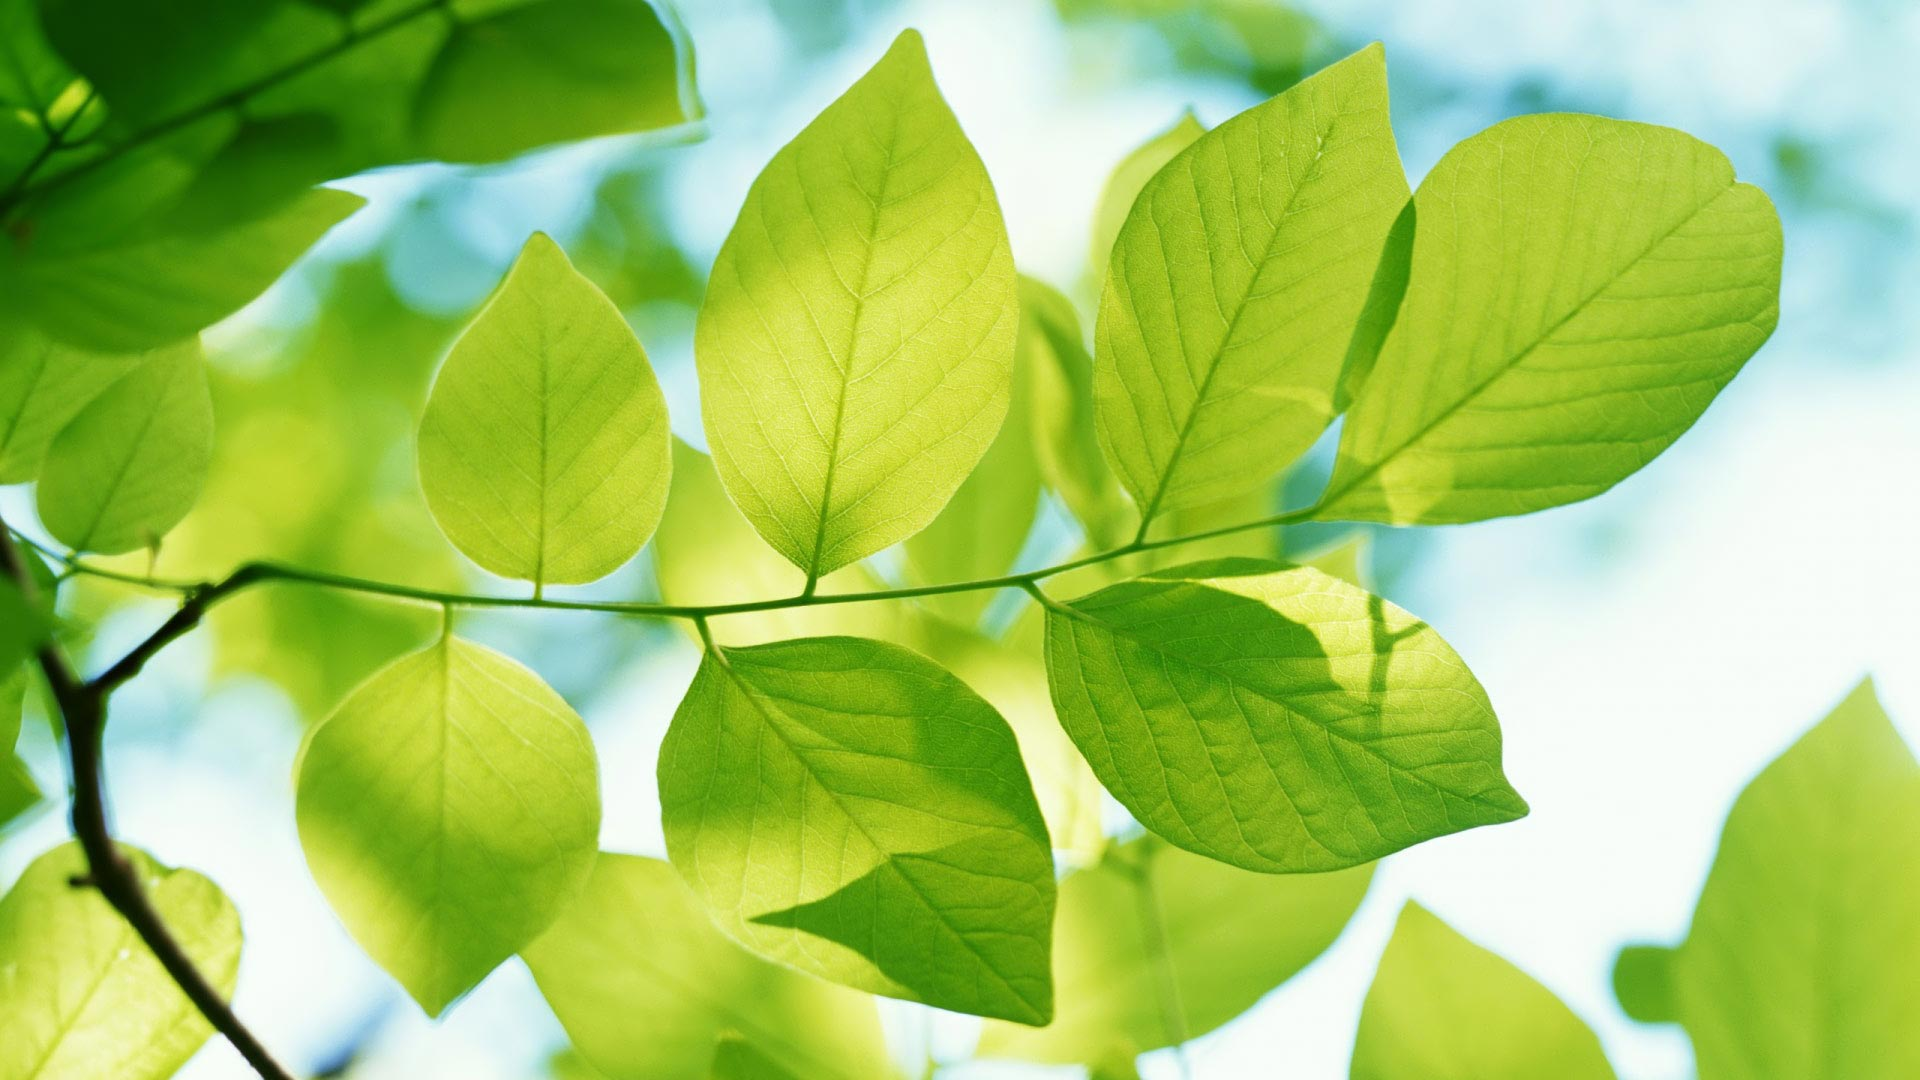
\includegraphics[width=0.5\textwidth]{./figures/translucent_leaves.jpg}
\end{center}
\caption[Fotografie průsvitných listů]%
{ Fotografie skutečných listů, kde se projevuje jejich průsvitnost, zdroj \cite{TLW} \label{fig:translucentLeaves}
}

\end{figure}

Metod a postupů, jak zobrazovat listy v real-time existuje několik. Většina přístupů se ale spokojuje s tím, že bere v potaz pouze povrchové vlastnosti listu a simuluje tak například členitost jeho povrchu či běžné odrazové vlastnosti. Metoda popsaná v \cite{Habel_2007_RTT} ovšem zahrnuje i průsvitnost listů, která hraje zásadní roli zejména na spodní straně listu (viz obr. \ref{fig:translucentLeaves}). Osvětlení listu lze zformulovat do následujícího vztahu
\begin{equation}
L = L_D + L_I + L_E,
\end{equation}
kde výsledné osvětlení $L$ z jednoho světelného zdroje se skládá z příspěvku přímého ($L_D$) a nepřímého ($L_I$) osvětlení a složky $L_E$, kterou list emituje. 
V následujícím textu bude rozebrán pouze příspěvek přímého osvětlení. Zbylé budou aproximovány ambientní složkou. Přímé osvětlení lze pak schematicky rozepsat jako:
\begin{equation}
\label{eq:directLight}
L_D = L_{diffuse} + L_{specular}+ L_{ambient} + L_{translucent},
\end{equation}
kde první tři členy představují příspěvek odraženého světla, zatímco poslední člen $ L_{translucent}$ se vztahuje k průsvitnosti listu.

K vyjádření difuzní a spekulární složky využijeme popisu z obrázku \ref{fig:lightModel}.
 \begin{figure}[here]
\begin{center}
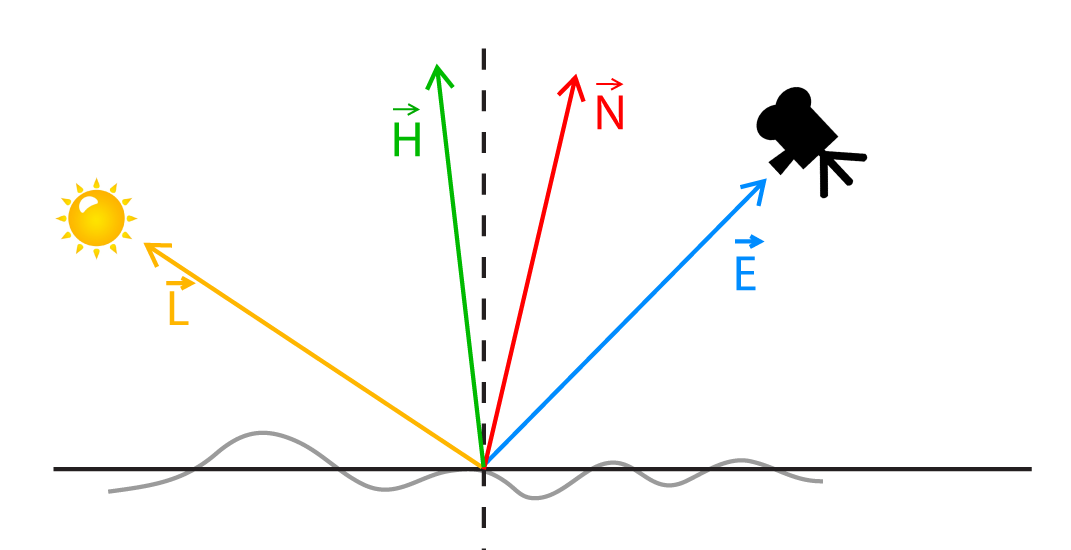
\includegraphics[width=0.5\textwidth]{./figures/lightModel.png}
\end{center}
\caption[Situace na povrchu listu]
{Situace na povrchu listu.  Vektor $\vec{N}$ definuje normálu v bodě dopadu paprsku. $\vec{E}$ udává směr k pozorovateli a $\vec{L}$ ke světlu. Vektor $\vec{H}$ je definován na ose úhlu mezi $\vec{L}$ a $\vec{E}$. Šedivá křivka představuje povrch.\label{fig:lightModel}
}
\end{figure}
Difuzní složku lze určit jako příspěvek světla vážený úhlem mezi přicházejícím paprskem světla $\vec{L}$ a normálou povrchu $\vec{N}$ v místě jeho dopadu:
\begin{equation}
L_{diffuse} = \vec{N} \cdot \vec{L}
\end{equation}
Výpočet spekulární složky je oproti tomu složitější. Nevyužívá Phongova osvětlovacího modelu, ale nahrazuje ho odvozeninou osvětlovacího modelu Cook-Torrance popsaného v \cite{Cook:1981:RMC:965161.806819} a \cite{Bousquet2005201}. Tento model pracuje s BRDF jež operuje nad proměnými $\vec{N}$, $\vec{L}$, $\vec{E}$, $\vec{H}$ (význam viz obr. \ref{fig:lightModel}), $\sigma$ udávajícím drsnost povrchu a indexem lomu $n$ světla na povrchu listu.

\begin{equation}
\label{eq:brdf}
BRDF_{spec}(\vec{N}, \vec{L}, \vec{E}, \vec{H}, \sigma, n) = \frac{R(\sigma, \vec{N}, \vec{H}) \cdot F(n, \vec{H}, \vec{E}) \cdot G(\vec{N}, \vec{L}, \vec{E},\vec{H}) }{(\vec{N}\cdot\vec{L})(\vec{N}\cdot\vec{E})\pi}
\end{equation}
Člen $R(\sigma, \vec{N}, \vec{H})$ představuje vliv hrubosti povrchu a může být vyjádřen jako:
\begin{equation}
\label{eq:roughness}
R(\sigma, \vec{N}, \vec{H}) = \frac{1}{\sigma^2 \cdot ( \vec{N}\cdot\vec{H})^4} \cdot e^{\left ( \frac{\frac{1}{ ( \vec{N}\cdot\vec{H})^2} -1}{\sigma^2}\right )}
\end{equation}
Naproti tomu, člen $F(n, \vec{H}, \vec{E})$ popisuje lesklou složku:
\begin{align}
\label{eq:fresnel}
c &= \vec{H} \cdot \vec{E} \nonumber\\
g &= \sqrt{n^2 + c^2 - 1}\nonumber\\
F(n, \vec{H}, \vec{E}) &= \frac{1}{2} \left ( \frac{g-c}{g+c} \right)^2 \left [  1+ \left( \frac{c (g+c)-1}{c(g-c)+1}\right)\right ]
\end{align}
Konečně člen $G(\vec{N}, \vec{L}, \vec{E},\vec{H})$ popisuje geometrii v bodě dopadu paprsku:
\begin{equation}
\label{eq:geometry}
G(\vec{N}, \vec{L}, \vec{E},\vec{H}) = \min{} \left( 1, \frac{2\cdot(\vec{N}\cdot\vec{H})\cdot(\vec{N}\cdot\vec{E})}{(\vec{E}\cdot\vec{H})}, \frac{2\cdot(\vec{N}\cdot\vec{H})\cdot(\vec{N}\cdot\vec{L})}{(\vec{E}\cdot\vec{H})} \right)
\end{equation}

Složka způsobená průsvitností listu má dominantní vliv, pokud se světelný zdroj nachází za rovinou listu vzhledem k pozorovateli. K jejímu vyjádření je použit BSSRDF model. Jeho konstrukcí a určením pro různé listy se věnuje \cite{Habel_2007_RTT} a tato problematika zde nebude dále rozebírána. Zmiňovaná funkce $L_t$ závisí na pozici $\vec{x}_0$, směru k pozorovateli $\vec{E}$ a směru ke světlu $\vec{L}$ a může být napsána v diskrétní formě takto:
\begin{equation}
\label{eq:bssrdf}
L_t(\vec{x}_0, \vec{E}, \vec{L}) = \rho_t(\vec{x}_0, \vec{E}) A_p \sum\limits_{\vec{x}_i} T(r, d(\vec{x}_i))E(\vec{x}_i, \vec{L}),
\end{equation}
kde $\rho_t(\vec{x}_0, \vec{E})$ reprezentuje propustnost, $A_p$ zastupuje plochu texelu, $T(r, d(\vec{x}_i))$ je dynamické konvoluční jádro díky závislosti na tloušťce listu $d(\vec{x}_i)$ a konečně $E(\vec{x}_i, \vec{L})$ je přenosová funkce osvitu (irradiance transport function). Jde v zásadě o proces konvoluce obrazové informace a můžeme tedy odlišit konvoluční část.
\begin{align}
\label{eq:bssrdf_convol}
L_t(\vec{x}_0, \vec{E}, \vec{L}) &= \rho_t(\vec{x}_0, \vec{E}) L_t^C( \vec{x}_0, \vec{L}) \\
L_t^C( \vec{x}_0, \vec{L})  &= A_p \sum\limits_{\vec{x}_i} T(r, d(\vec{x}_i))E(\vec{x}_i, \vec{L}),
\end{align}
 Právě konvoluční část tvořená hemisférickou funkcí $L_t^C$ je v real-time příliš obtížné vypočíst, a proto se předpočítá pro každý texel. Reprezentována pak je pomocí tzv. \emph{Half Life 2 bází} (HL2b). Jde o konstrukt, který umožňuje jednoduše vyjádřit reprezentovanou funkci pro daný hemisférický směr. Bázové vektory HL2b jsou následující:
\begin{align}
\label{eq:hl2b_vectors}
\vec{H}_1 &= (-\frac{1}{\sqrt{6}}, -\frac{1}{\sqrt{2}}, \frac{1}{\sqrt{3}}) \nonumber\\
\vec{H}_2 &= (-\frac{1}{\sqrt{6}}, \frac{1}{\sqrt{2}}, \frac{1}{\sqrt{3}}) \nonumber \\
\vec{H}_3 &= (\sqrt{\frac{2}{3}}, 0, \frac{1}{\sqrt{3}})
\end{align}
Tyto vektory pak definují tři kosínové bázové funkce na polokouli (hemisféře):
\begin{equation}
\label{eq:hl2b_cosineFunctions}
\mathcal{H}_i(\vec{d}) = \sqrt{\frac{3}{2\pi}}\vec{H}_i \cdot \vec{d}
\end{equation}
Hemisférickou funkci $f(\vec{d})$ pro směr $\vec{d}$  lze tedy přepsat pomocí těchto bázových funkcí následovně:

\begin{equation}
\label{eq:hl2b_function}
f(\vec{d}) = \sum\limits_{i=1\dots3}h_i\mathcal{H}_i(\vec{d}),
\end{equation}
kde $h_i$ jsou souřadnice vzhledem k bázovým funkcím.

Výsledný vztah rekonstruující původní $L_t$ využívající HL2b pro předpočítanou konvoluční funkci pak vypadá takto:
\begin{equation}
\label{eq:hl2b_use}
L_t^R(\vec{x}_0, \vec{L}) = L_D \rho(\vec{x}_0) \sum\limits_{i=1\dots3}h_i(\vec{x}_0)\sqrt{\frac{3}{2\pi}}\vec{H}_i \cdot  \vec{L}
\end{equation}
Uvážíme-li, že $L_D \rho(\vec{x}_0)$ a $h_{1\dots3}(\vec{x}_0)$ lze uložit do textur (pro pozici $\vec{x}_0$), lze tím pádem průsvitnost vypočíst na základě pouze dvou dotazů do textur.

Posledním krokem je přizpůsobit výše popsané postupy tak, aby bylo možné dynamicky měnit barvu listů. Barva se liší jednak v rámci jednoho listu, jednak mezi listy. Sezónní změny barvy listu se často projevují různě v různých částech listu. Zatímco okrajové části mohou být už červené či žluté, středové části mohou zůstávat stále zelené. Toto chování ovšem není cílem napodobit. Důraz bude kladen na celkovou barevnost listu, která hraje roli při pohledu z větší vzdálenosti.
\begin{figure}[here]
\begin{center}
$\begin{array}{cc}
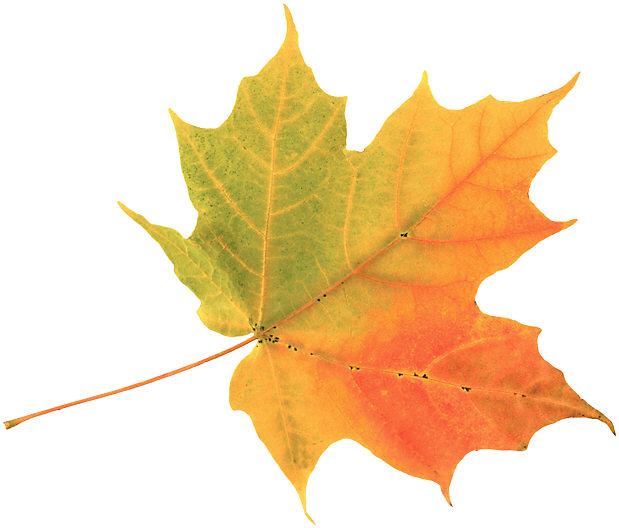
\includegraphics[width=0.4\textwidth]{./figures/fall-leaf.jpg}&
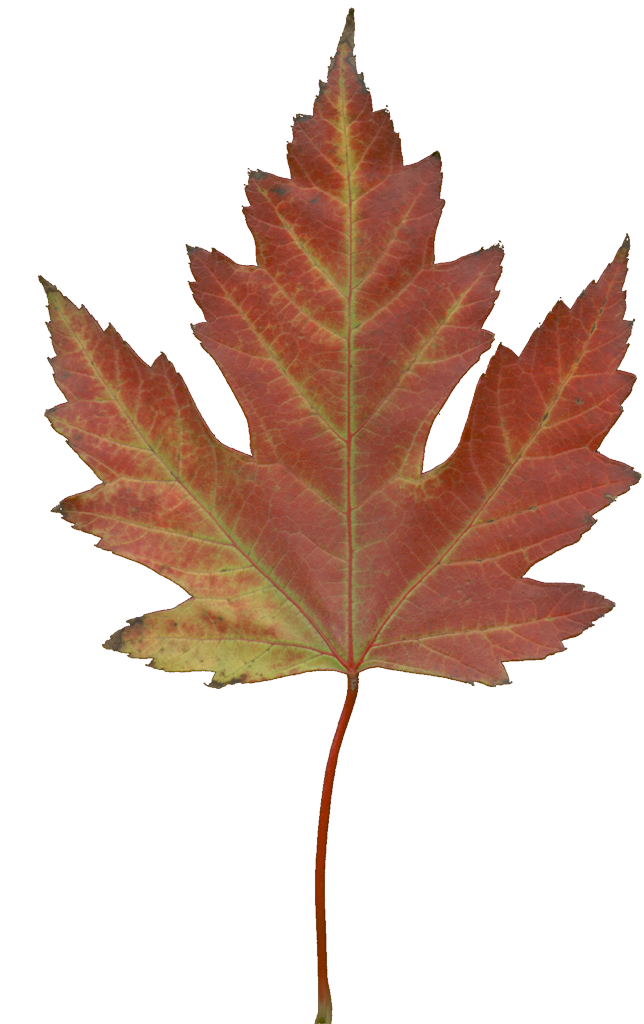
\includegraphics[width=0.3\textwidth]{./figures/fall-leaf2.png}
\\
(a)&(b)
\end{array}$
\end{center}
\caption{ Fotografie skutečných listů, barevné variace v ploče listu\label{fig:fallLeaves}
}
\end{figure}

Vyjdeme-li ze vztahu \ref{eq:directLight}, a budeme-li ho chápat pouze jako jednotlivé skalární podíly intenzit světla, můžeme vytvořit následující vztah pro zahrnutí barevnosti listu: 
\begin{equation}
\label{eq:color_solution}
L_D = L_{diffuse}  \mathcal{D} + L_{specular} \mathcal{S} + L_{ambient} \mathcal{A}   + L_{translucent} \mathcal{T} ,
\end{equation}
přičemž $\mathcal{D}$ je difuzní barva v daném bodě, $\mathcal{S}$ je barva odlesku daná barvou světelného zdroje a materiálem, $\mathcal{A}$ je barva ambientního příspěvku světla a $\mathcal{T}$ je barva vzniklá průchodem světla listem.

 Pro konkrétní bod $x$ a sezónu $s$ lze barvy vyjádřit jako:
\begin{align}
\label{eq:color_def}
\mathcal{D}(x,s) &= (c_v(x) + c_s(s))\cdot \mathcal{M}_{diffuse}\nonumber\\
\mathcal{A}(x,s) &= (c_v(x) + c_s(s))\cdot \mathcal{M}_{ambient}\nonumber\\
\mathcal{S}(x,s) &= \mathcal{M}_{specular}\nonumber\\
\mathcal{T}(x,s) &= (c_t(x) + c_s(s))\cdot \mathcal{M}_{translucent} ,
\end{align}
kde $ \mathcal{M}_{(\dots)}$ je pro daný materiál na světelný zdroj konstanta, $c_v(x)$ je prostá barva listu, která je definovaná texturou, $c_s(x)$ je barevná odchylka daná sezónními změnami barvy (dovolíme si zjednodušení: sezónní barevná odchylka je pro celý list stejná ). Člen $c_t(x)$ vyjadřuje barvu po průchodu světla listem, která je rovněž definovaná texturou. Na tomto místě je dobré přiznat, že správnější by bylo uvažovat pro různé barevné variace listu dané sezónou i různé barvy průsvitné složky. Řešní by se tím ovšem zkomplikovalo a i popsaný přístup funguje relativně dobře.
Předpokládá se, že každá ze dvou stran listu bude vyhodnocována odděleně s jinými parametry (různé textury, příp. materiály). Na obrázku \ref{fig:leafResources} jsou zdrojové textury pro jednu stranu listu.
\begin{figure}[here]
$\begin{array}{cccc}
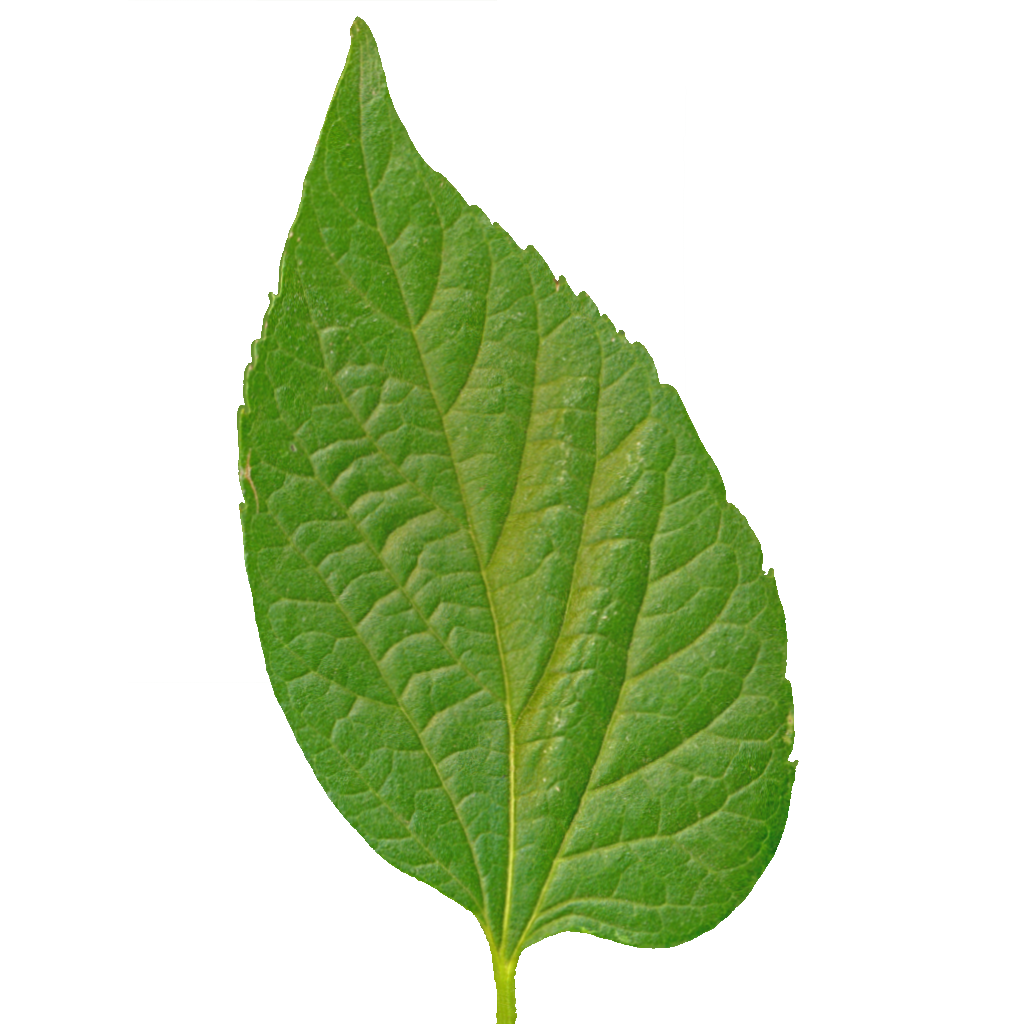
\includegraphics[width=0.2\textwidth]{./figures/leaf3_decal_front.png}&
&
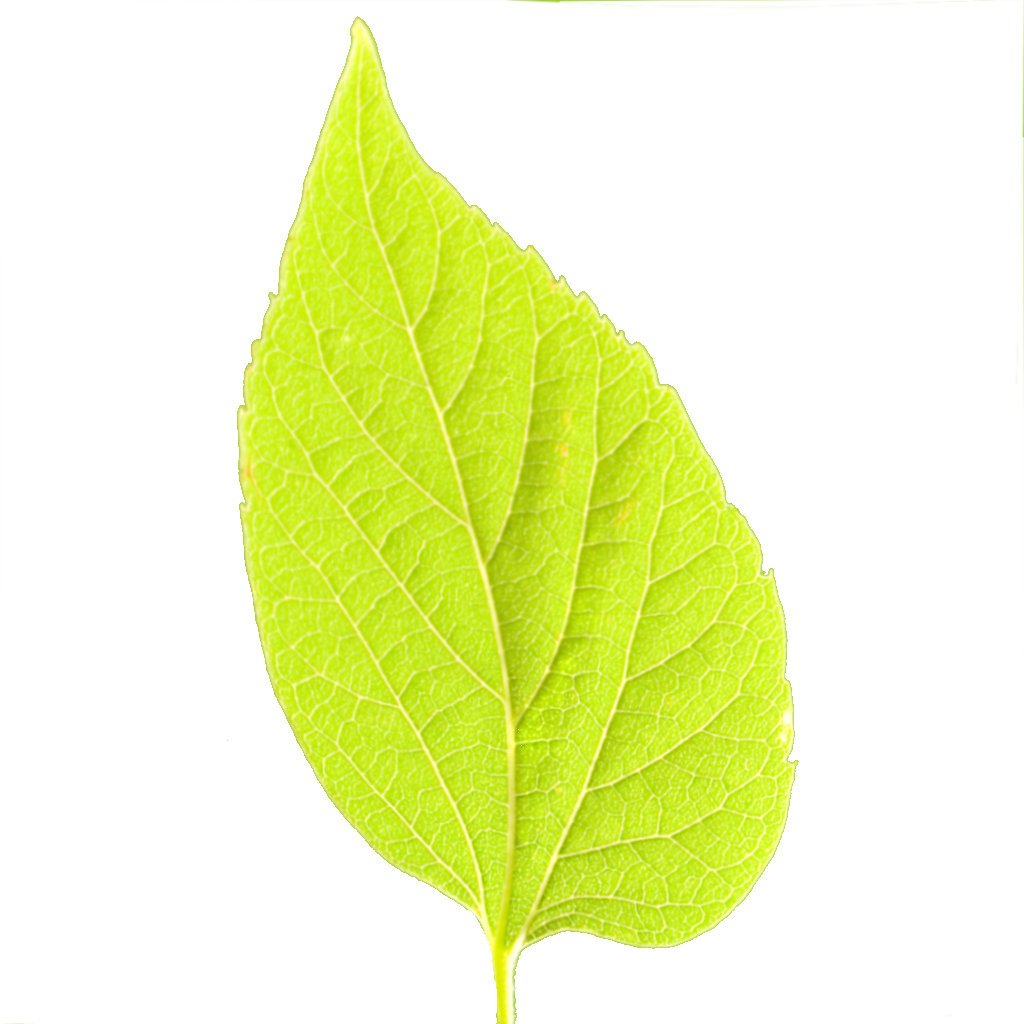
\includegraphics[width=0.2\textwidth]{./figures/leaf3_translucency_front.png}&
\\
(a)&&(b)&
\\
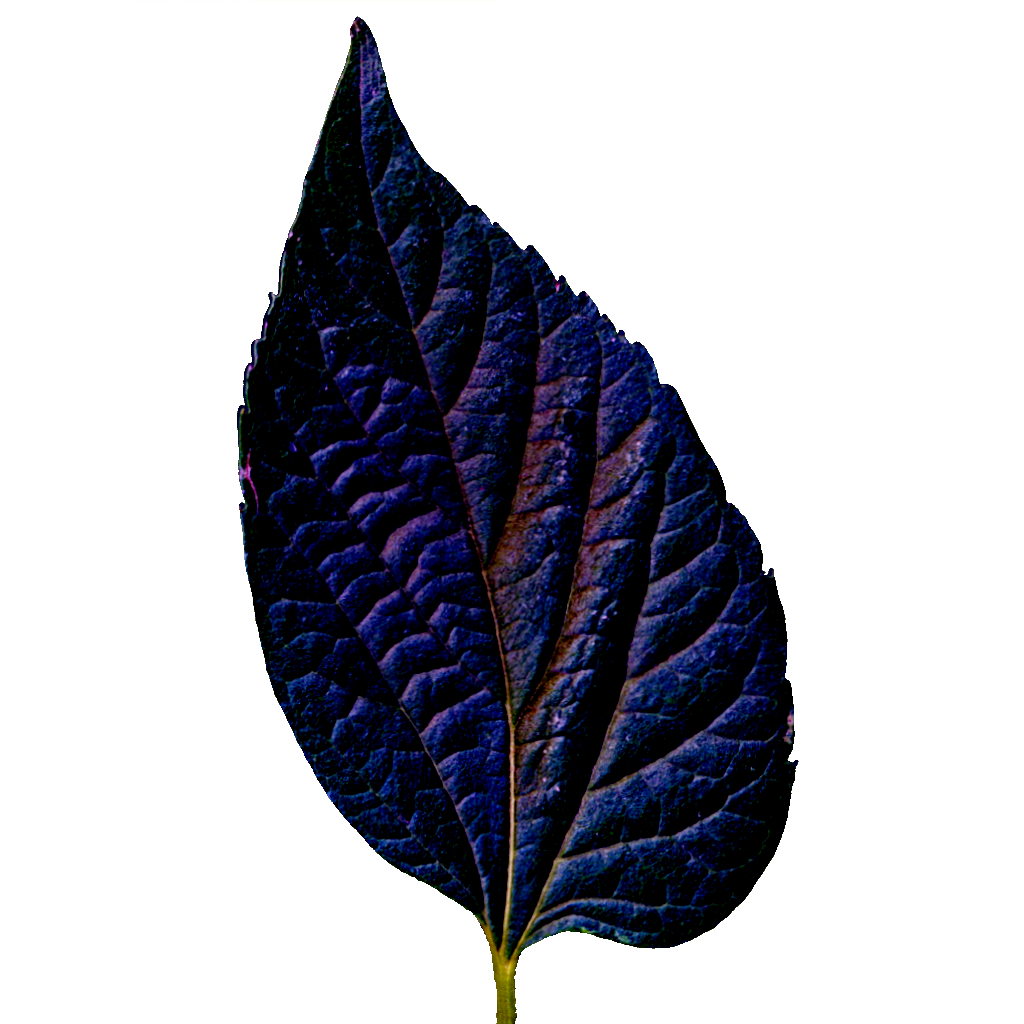
\includegraphics[width=0.2\textwidth]{./figures/leaf3_decal_front_e.png}&
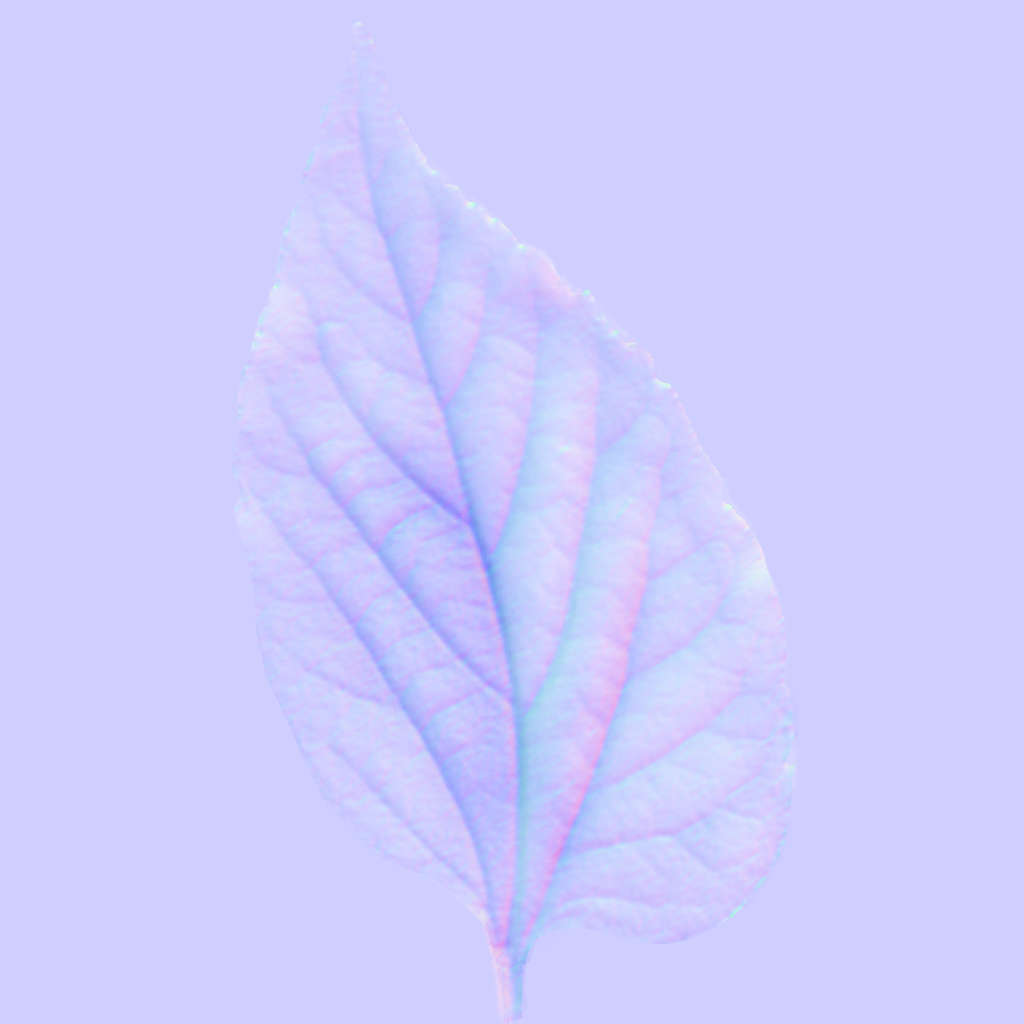
\includegraphics[width=0.2\textwidth]{./figures/leaf3_normal_front.png}&
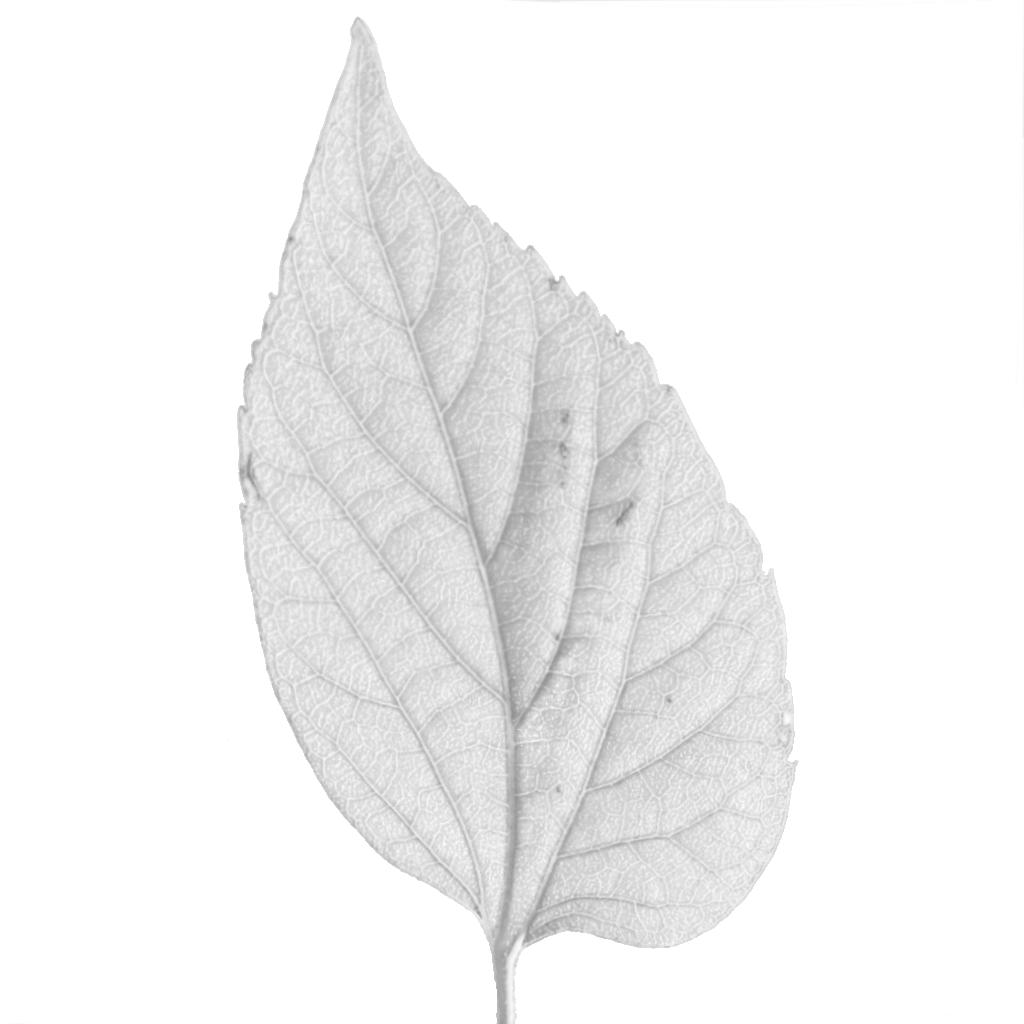
\includegraphics[width=0.2\textwidth]{./figures/leaf3_translucency_front_e.png}&
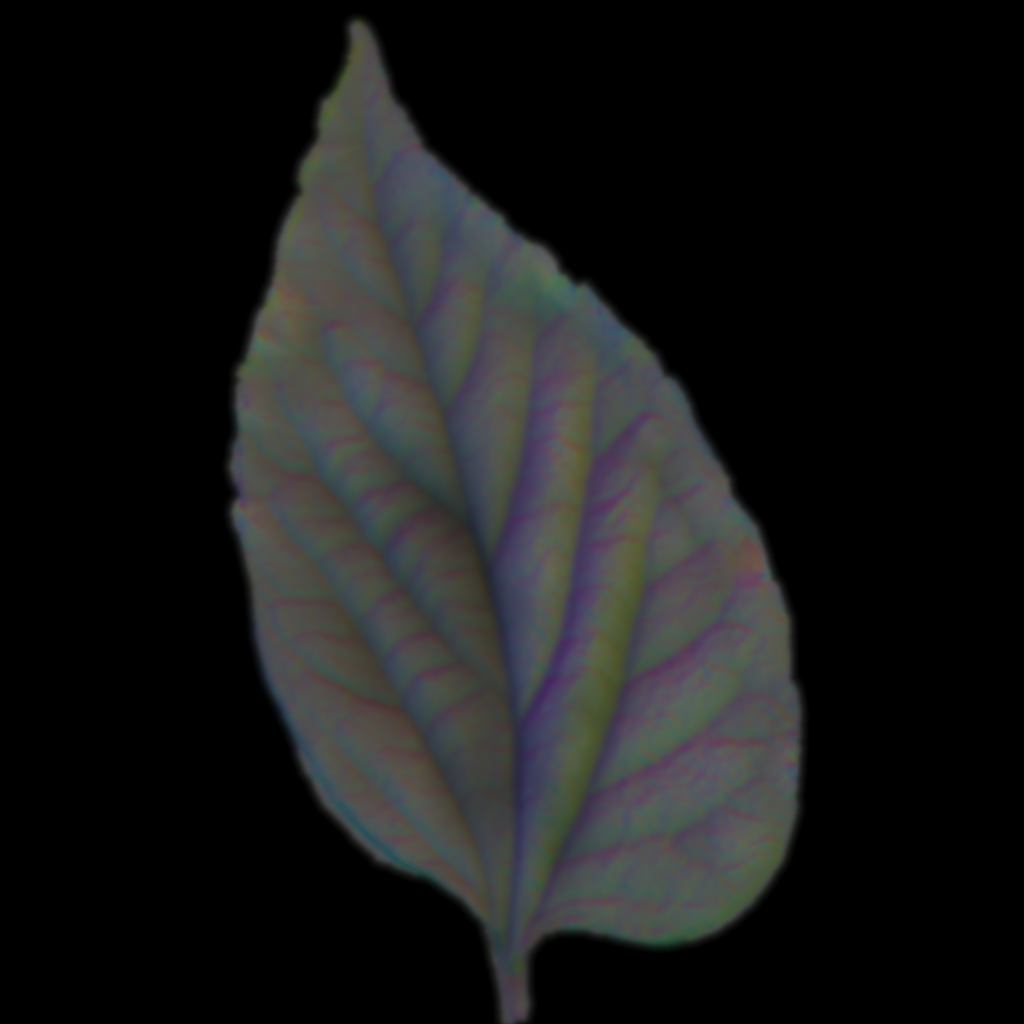
\includegraphics[width=0.2\textwidth]{./figures/leaf3_halflife2_front.png}
\\
(c)&(d)&(e)&(f)
\end{array}$
\caption[Zdrojové textury pro výpočet osvětlení listů]%
{Zdrojové textury pro výpočet osvětlení listů. (a) původní barevná mapa, (b) původní mapa průsvitnosti, (c) mapa barevných odchylek od základní barvy listu (pro názornost zvětšeny), (d) normálová mapa, (e) mapa průsvitnosti, (f) mapa koeficientů Half Life 2 bázových funkcí \label{fig:leafResources}
}
\end{figure}
Pro listy jsou ovšem k dispozici původně jiná zdrojová data. Původní barevná mapa obsahuje prosté barvy listu (např. fotografie) - jde vlastně o záznam podoby listu pro jednu sezónní barvu a tu neumožňuje přímo a jednoduše dynamicky měnit. Mapu barevných odchylek můžeme získat z původní barevné mapy odečtením základní barvy listu (později přičtena jako sezónní barva listu). Obdobné předzpracování je nutné provést s původní mapou průsvitnosti, na kterou je výhodnější nahlížet jako na mapu intenzit.  

\newpage